\chapter{Machine learning and statistical methods}
\label{chapter:MLStat}

This Chapter introduces the Machine Learning (ML) methods used in the different analysis to enhance the separation between the signal and the background, and also the statistical methods used to extract the measurements of the signal.\\

\acrlong{MLlabel}~(\acrshort{MClabel}) is one of the core developing fields in computer science allowing the analysis of large and complex datasets, offering sophisticated techniques with a broad range of possible applications. Regarding high energy physics, the large amount of \acrshort{MClabel} simulations or data that is being recorded is well suited for the application of \acrshort{MLlabel} techniques. In this chapter, different multi-variate techniques used in this thesis are introduced, focusing on the classification methods used to improve signal and background separation.\\

In order to test the predictions of a given model, experimental data and \acrshort{MClabel} simulations are compared using statistical methods. This chapter describes the tools used to extract a measurement of the production of the target signal, in addition to upper limits.

\section{Machine Learning}

The deployment of \acrshort{MLlabel} methods is already reaching crucial tasks in \acrshort{ATLASlabel} as online data recording, from neural networks in calorimetry FPGAs~\cite{Laatu:2022fni} to particle reconstruction in trigger algorithms~\cite{ATLAS:2019uhp}, which benefit from faster and more efficient response than previous filters.\\

For those cases, a neural network is trained to reduce background--signal ratio, to offer a high-level discriminating variable for a classification problem or to provide a prediction of a certain quantity. These methods can outperform conventional algorithms as the inference is performed from multi-dimensional inputs, providing large amounts of information to the machine learning algorithm. Regular algorithms rely on kinematic variables and although multiple can be combined, \acrshort{MLlabel} methods can use a greater amount of inputs and reach higher performance, given enough data.\\

Regarding detector simulation, it is one of the most computational intensive tasks within \acrshort{ATLASlabel}, especially from the calorimeter simulation, and solutions involving adversarial networks and auto-encoders are being studied to output faster but reliable output.\\

Regarding particle reconstruction and identification, examples of implementations can be found within the $\tau$ identification~\cite{ATLAS:2019uhp} or $b$-tagging algorithms~\cite{ATL-PHYS-PUB-2020-014}. In physics analyses, the use of \acrshort{MLlabel} is already standardised to typically reconstruct signal processes or to discriminate them from the background. Then, the output is a high discriminating variable that can be used to define high-purity signal analysis regions, for example.\\

Machine Learning is a very broad umbrella term for algorithms which are not per se optimised for a specific task but are can adapt to different problem sets by tuning their parameter set using data (training).
\acrshort{MLlabel} requires, besides the model itself, preparation and follow-up processing steps. In which extent they are necessary depends on the available data, the model and its application.\\

Generally, two types of machine learning are distinguished: Supervised learning and Unsupervised learning. The main difference is that the first requires fully labelled training data while the latter does not. In the context of this thesis, supervised approaches are used based on Neural Networks (NNs) and Boosted Decision Trees (BDTs).\\

The statistical model is denoted as $\text{P}_\text{model}(\mathbf{x_i}; \boldsymbol{\theta})$ parameterised with the set of parameters $\boldsymbol{\theta}$ while $\mathbf{x_i}=(x_i^1,x_i^2,...,x_i^M)$ is the feature set of a single input data point $i$ of the $\mathbf{X}=(\mathbf{x_1},\mathbf{x_2},...,\mathbf{x_N})$ dataset consisting of $N$ data points. $\text{P}_\text{data}$ is the true distribution that generates the data but is unknown. In the case of supervised learning, every data point has a label which categorizes the event, $\mathbf{y}=(y_1,y_2,...,y_N)$.

\subsection{Pre-processing}

The selection of the dataset and its size depends on the problem that the \acrshort{MLlabel} is intended to solve. The datasets used in \acrshort{MLlabel} methods to discriminate between signal and background processes usually consist on simulated events. If the aim is to reconstruct a specific quantity, only the events of the target signal are used. Aside, the dataset can also consist of just objects, like $b$-jets, instead of events. The dataset and the amount of input depends mostly then on the problem at hand, its complexity and the target performance, as more complex setups will need advanced algorithms with higher number of input variables and large datasets.\\

The input variables can be categorised as low- or high-level variables. The low-level variables are usually available quantities that have not been combined or designed to directly help to the problem, like the kinematics of the objects of an event. Then, high-level variables are referred to those obtained with low-level variables and designed to offer discrimination, as reconstructed kinematics or the output of other classifiers, like $b$-tagging. Although high-level variables offer a lot of discrimination, a complete set of low-level variables have the necessary information to reach or even surpass the same level of discrimination, as low correlations between variables can be exploited in advanced setups.\\

It is important to ensure an unbiased training process. For this purpose, the full dataset is split at least in two orthogonal samples. The training sample is used for the actual algorithm training, while the validation set is evaluated and monitored to choose between different models. While a loss function is used to find the best parameter set for the training itself, the performance on the validation set is evaluated in terms of sensitivity, selection efficiency, stability... in order to fine-tune the model, such as the choice of input variables or hyperparameters. Ideally, a third dataset referred to as testing set is only used to evaluate the final algorithm and is not involved in the training process. Some trainings performed in this thesis are not performed with the testing set although no significant bias is introduced, as the difference in performance between the validation and testing set is below statistical effects. In order to evaluate the full dataset, cross-validation (also named $k$-folding~\cite{EncyclopediaofML}) setups are used where $k$ trainings are performed where the train/validation/test sets are labelled accordingly so every set can be evaluated appropriately.\\

In this thesis and typically in \acrshort{ATLASlabel} analyses, every simulated event has an associated unique integer not correlated with any physical variable. Hence, it is ideal to split the full dataset into the different sets. Another detail is that every simulated event has an event weight, so the full simulated process has the appropriate cross-section and kinematic distributions, which value can also be negative in some cases. This is almost exclusive of high energy physics datasets and although the user level tools accept event weights as input, the absolute value of the even weights has to be used as negative values are not properly defined in the training. 

\subsection{Performance}

The model performance is usually the decisive measure of an \acrshort{MLlabel} method and depending on the objective, different metrics are used to better evaluate the performance. The most common variables are discussed in the following.

\subsection{Loss function}

The loss function $E$ or cost function is the quantity optimised during the model training and represent the deviation of a model from the desired behaviour. To be suitable for minimisation, the function has to be differentiable. The choice of the loss function depends on the problem and requires optimisation. For supervised learning, the loss function depend on the labels and the worse the prediction is, the higher the loss function.\\

It is standard to express the loss of the full dataset $\mathbf{X}$ as the average of loss of the single data points $\mathbf{x_i}$,

\begin{equation}
    E(\mathbf{X},\boldsymbol{\theta})=\frac{1}{N}\sum_{i=1}^NE(y_i,\text{P}_\text{model}(\mathbf{X},\boldsymbol{\theta}))
\end{equation}

For regression problems the typical expression is the mean square error~\cite{EncyclopediaofML}, 

\begin{equation}
    E_{MSE}(\mathbf{X},\boldsymbol{\theta}) = \frac{1}{N}\sum_{i=1}^N (y_i\text{P}_\text{model})^2
\end{equation}

simply an average of the deviation from the true labels. For binary classification, the so-called \textit{binary cross-entropy}~\cite{binarycross} is frequently used, 

\begin{equation}
    E_{BSE}(\mathbf{X},\boldsymbol{\theta}) = -\frac{1}{N}\sum_{i=1}^N y_i\cdot\log(\text{P}_\text{model}(\mathbf{X},\boldsymbol{\theta}))+(1-y_i)\cdot\log(1-\text{P}_\text{model}(\mathbf{X},\mathbf{X}))
\end{equation}

which is the negative log-likelihood of a Bernouilly distribution, and a modified version is used in multi-classification problems. 

\subsubsection{AUC}

In the analyses presented in this thesis, the output distribution of the NN is used as a high-level variable and in the  multi-variate fit to data. Hence, the loss function is not the only important criteria as both the shapes and the separation between the signal and background output distributions are essential for the performance of the analyses. The quantity to evaluate the separation from signal and background for a given variable is the \textit{Area Under the ROC Curve} (AUC), and is the main decisive variable for a training in this thesis.\\

Given two variable distributions from a signal and a background sample, the \textit{ROC} curve (Receiver Operating Characteristic) is defined as the signal efficiency against the background rejection.%\todo{prepare graph?}
The shape of the curve already provides a lot of the information regarding the overlap of the distributions, but the characteristic quantity is the integral of the curve, the AUC. The AUC minimum value is 0.5, when the overlap between two distributions is total, while the maximum value is 1, when the distributions are totally separated. In the maximum value case, there is a cut in the discriminating variable can distinguish completely between signal and background.

\subsection{Neural networks}
\label{ML:SectionNN}
Neural Networks (NNs) were introduced in the 1940s~\cite{McCulloch1943} but became feasible in the last decades as large computing power and GPUs are widely available. The concept of a NN are nodes (neurons) connected to each other via weights, and the most basic network is referred as feed-forward NN.\\

An example is illustrated in Figure~\ref{ML:normalNN}, with in one input layer, one hidden layer and one output node. The result of node has the form of a linear system $b+w\cdot x$, with bias $b$, weight $w$ and the input of the neuron $x$. More technically, the result of every node (except the input layer) is given by the sum of its inputs, the output of the different neurons connected to the given node multiplied by the weights $w_i$ which represent said connection. More generally, a bias $b_i$ is added to the sum and then used as input to an activation function $f_i$, which introduces non-linearity. The final output of the depicted feed-forward NN can be expressed as

\begin{figure}[htbp]
    \RawFloats
    \begin{center}
    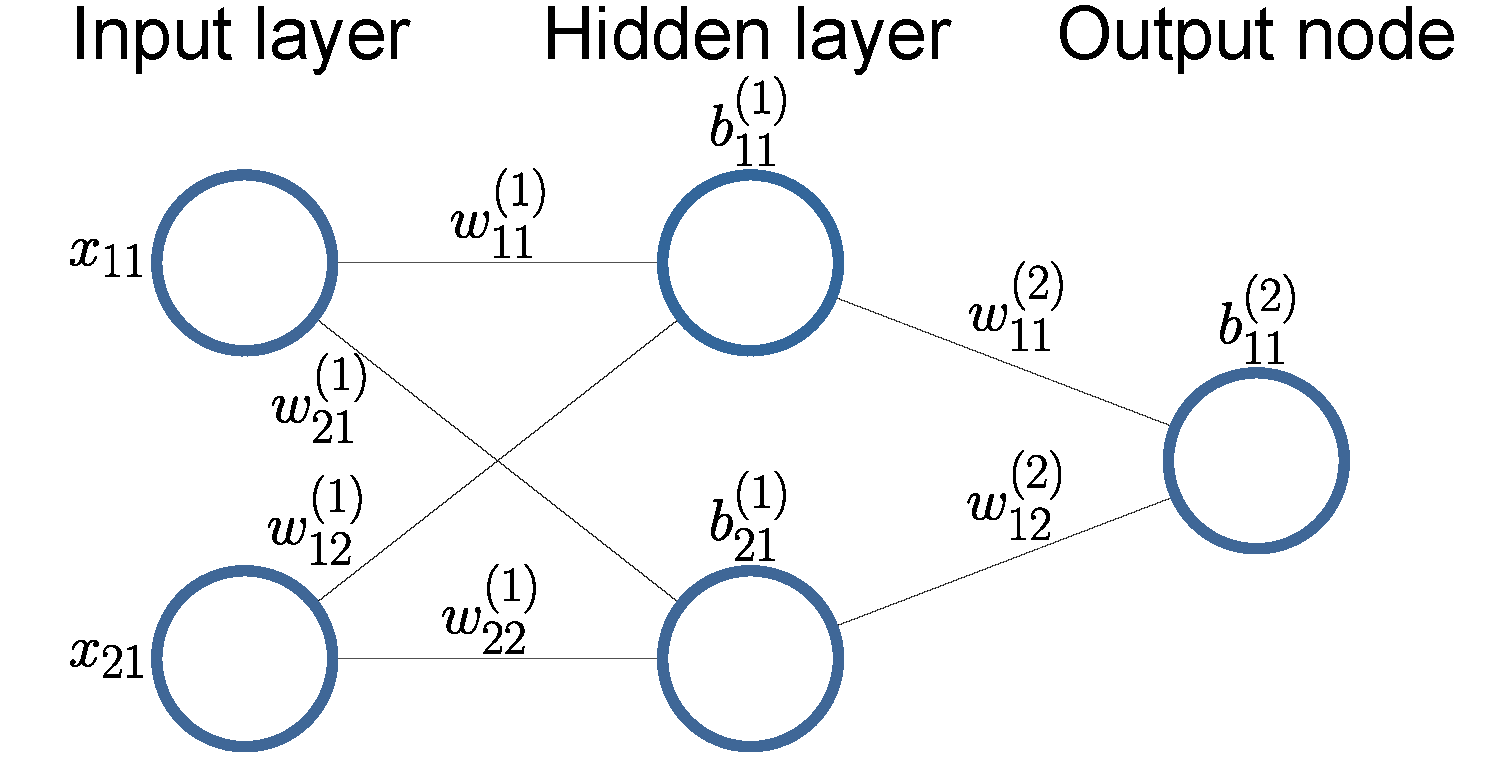
\includegraphics[width=0.75\textwidth]{ML/nnnormal.pdf}
    \caption{
        Fully connected feed-forward neural network with two input nodes, one hidden layer with two nodes and one output node.
    }
    \label{ML:normalNN}
    \end{center}
\end{figure}

\begin{equation}
    \text{P}_\text{model}(\mathbf{X},\boldsymbol{\theta}) = f_2(\mathbf{b_2}+\mathbf{W_2}f_1(\mathbf{b_1}+\mathbf{W_1}\mathbf{x}))
\end{equation}

with the inputs of a given data-point $\mathbf{x}$; the parameter set $\boldsymbol{\theta}$ including weight matrices $W_i$ and bias terms $b_i$. Fully expanding in matrix notation,

\begin{equation}
    \text{P}_\text{model}(\mathbf{X},\boldsymbol{\theta}) = f_2\left( \begin{bmatrix} b_{11}^2 \end{bmatrix}+ \begin{bmatrix} w_{11}^2 & w_{12}^2\end{bmatrix}f_1\left( \begin{bmatrix} b_{11}^1 \\  
                                                            b_{21}^1  \end{bmatrix}+ \begin{bmatrix} 
    w_{11}^1 & w_{12}^1 \\ 
    w_{21}^1 & w_{22}^1\end{bmatrix} \begin{bmatrix}
        x_{11}\\
        x_{21}
    \end{bmatrix} \right) \right)
\end{equation}

This simple example has nine free parameters $\boldsymbol{\theta}$ which are optimised during the training; more complex networks easily reach several ten-thousands of free parameters. Due to the non-linearity introduced by $f_i$, a NN can approximate any arbitrary function by giving the network enough freedom (amount of hidden layers and nodes). When a NN consists of multiple hidden layers, it is referred as a deep learning~\cite{Goodfellow-et-al-2016} algorithm.\\

The main NN structure used in this thesis are feed-forward networks, but there are a vast number of different architectures available developed for very different applications~\cite{livingreview}. Several software packages are available and accessible to the public,  mainly in Python, with popular examples as Pytorch~\cite{NEURIPS2019_9015}, Tensorflow~\cite{tensorflow2015-whitepaper} and Keras~\cite{chollet2015keras}. The main package used in this thesis is the latter, which models are deployed in \acrshort{ATLASlabel} using the C++ based package lwtnn~\cite{lwtnn}.\\

The training of a NN is the process consisting on the optimisation of the free parameters $\boldsymbol{\theta}$ using gradient descent. Other parameters that affect the model and are manually set are called hyperparameter, which include for example the number of layers and nodes.\\

Regarding training, batch training is the typical procedure, where the minimisation of the loss function is done in steps with the training data divided into equally sized segments. The loss function is calculated, and the parameters optimised at every step. When a full iteration over the entire dataset is referred as an epoch. This method enhances the minimisation of the loss function as computing it using the full training dataset leads to profile the very specifics of the training dataset, hence loosing generalisation when evaluating other data not used in the training (overtraining), and can also lead to stop the minimisation process in local minima thus not reaching the true performance.\\

For batch training approach, the dataset is randomised and then split with an adequate batch size to ensure that every batch is a correct representation of the dataset. Hence, the batch size is a hyperparameter and if too small, the minimisation is faster but the loss function will vary too much at every step, leading to a lower resolution and lower performance, as the model will be too general. 

\subsubsection{Optimiser}

After a first random initialisation of the free parameters $\boldsymbol{\theta}$, they are updated iteratively at each step of the training following,

\begin{equation}
    \theta' = \theta - l \nabla_\theta E(\theta;\mathbf{X})
\end{equation}

where $l$ is the learning rate, also a hyperparameter, that tunes the rate of the update on the weights, the gradient of the loss function with respect the given free parameter. A large value of $l$ prevents the optimal convergence as the loss value might change enough between steps and the minimisation becomes random before reaching the minimum. On the other side, a very low learning rate slows the optimisation and the minimisation can get stuck in a local minimum. Methods that vary the learning rate or the batch size at every step can prevent the extremes and gradually shift to a precise approach with the number of steps or epochs~\cite{LRBatchSize}. In this thesis, the Adam optimiser~\cite{Kingma2015AdamAM} is used which estimates of the first and second moment of the gradient.

\subsubsection{Backpropagation}

For the gradient-descend method, the computation of the gradient of the loss function with respect to all trainable parameters is needed. However, it is not feasible to calculate it analytically for NNs as the gradient includes lots of nested gradients. Backpropagation~\cite{Rumelhart1986} is used to calculate the gradient, which computes the nested gradients applying the chain rule gradually to fully compute the network. The gradient computation is optimised by reusing sub-expressions and parameter dependencies.

\subsubsection{Activation Functions}

The introduction of activation functions $f(z)$ is essential to allow the NNs to act as a non-linear function. Many candidates of activation functions exist, from simple step functions to monotonically increasing functions (as $\tanh$) or logistic functions (as the \textit{sigmoid} function). Although these activation functions are simple and manage to harmonise the inputs of a node, the resulting NN suffers from vanishing gradient issues which significantly slow the training. The \textit{Rectified Linear Unit} ($\textsc{ReLU}$)~\cite{relu} activation function is widely used, defined as

\begin{align}
    f_\textsc{ReLU}(z)= \begin{cases}
            0& \text{for}  z<0 \\
            z& \text{for}  z\geq0\\
            \end{cases}\qquad f'_\textsc{ReLU}(z)= \begin{cases}
                0& \text{for}  z<0 \\
                1& \text{for}  z\geq0\\
                \end{cases}
\end{align}

which is not affected by vanishing effects and the gradient is fast to compute, as the derivative function $f'(z)$ is very simple. Other popular activation functions are the Leaky $\textsc{ReLU}$~\cite{lrelu} and \textit{Softplus}~\cite{Maas2013RectifierNI}.\\

In general, the output nodes have different activation functions depending on the desired shape of the result. For the classification problems, like the NN used in the thesis, the output node can be interpreted as a probability with the sigmoid function,

\begin{equation}
    f_\text{sigmoid}(z)=\frac{1}{1+e^{-z}}
\end{equation}

\subsubsection{Regularisation}

Besides the training performance, the ML model should be resilient to fluctuations in the training data or by the randomness of the training process itself. If performing the training with two equivalent data-sets results in very different models and performance, it might be a strong indication of overfitting or other instabilities, difficult to study as a NN has many free parameters.\\

To protect the model and its ability to be generalisable, the training is made robust with regularisation techniques. Most popular stochastic methods~\cite{JMLR:v15:srivastava14a,batchnorm,earlystop} are introducing dropout, batch normalisation or early stopping. The first, randomly removes an adjustable percentage (hyperparameter) of weights between neighbouring layers avoiding strong correlations between neurons. The batch renormalisation consists on scaling the input of the layers and the early stopping halts the training process after a criterion to avoid overtraining, like that the loss in the validation set is not improving after a certain amount of epochs.\\

Another popular method, the L2 regularisation, consists in adding a term in the loss function that includes the sum of the squared weight values, penalising large weight values. In this thesis, the dropout and early stopping are applied as textbook, while no effects were seen when introducing other methods like L2 regularisation. The batch normalisation is not applied, although an equivalent approach is applied to the input layer. The different input variables are scaled to have a mean value of 0 and a variance of 1, which avoids large differences in weights due to the difference of units. One consideration is that distributions like \pT\ are not bounded like $\eta$ and outliers at the tail of the distributions can introduce instabilities in the model.

\subsubsection{Neural network parameterisation}

The analyses presented in this thesis use a NN technique referred as parameterisation, usually applied to NN with signal or background events generated with different parameters. The parameterised NN~\cite{Baldi_2016} appears as a structure that simplifies trainings setups as it can replace sets of classifiers trained at individual values of given parameters, thus also increasing the statistics of the training dataset.\\

The NN has in the input layer these parameters that distinguish different classes of interest, like the training label set, a generator parameter or a source of uncertainty~\cite{Ghosh_2021}. Consequently, the response depends on the introduced parameters as depicted in Figure~\ref{ML:PNN}.\\

In the different searches presented in the thesis, the true mass of the targeted new BSM particle is used as a parameter. As the parameter can be used to directly classify the events, the training should be setup appropriately. For signal events the parameter corresponds to the mass of the corresponding sample, while for background it is not well-defined and a random value is assigned to each event, taken from the distribution of signal masses. This makes the NN not to directly use the parameter to perfectly classify the events, while the classification is optimised for each signal.

\begin{figure}[htbp]
    \RawFloats
    \begin{center}
    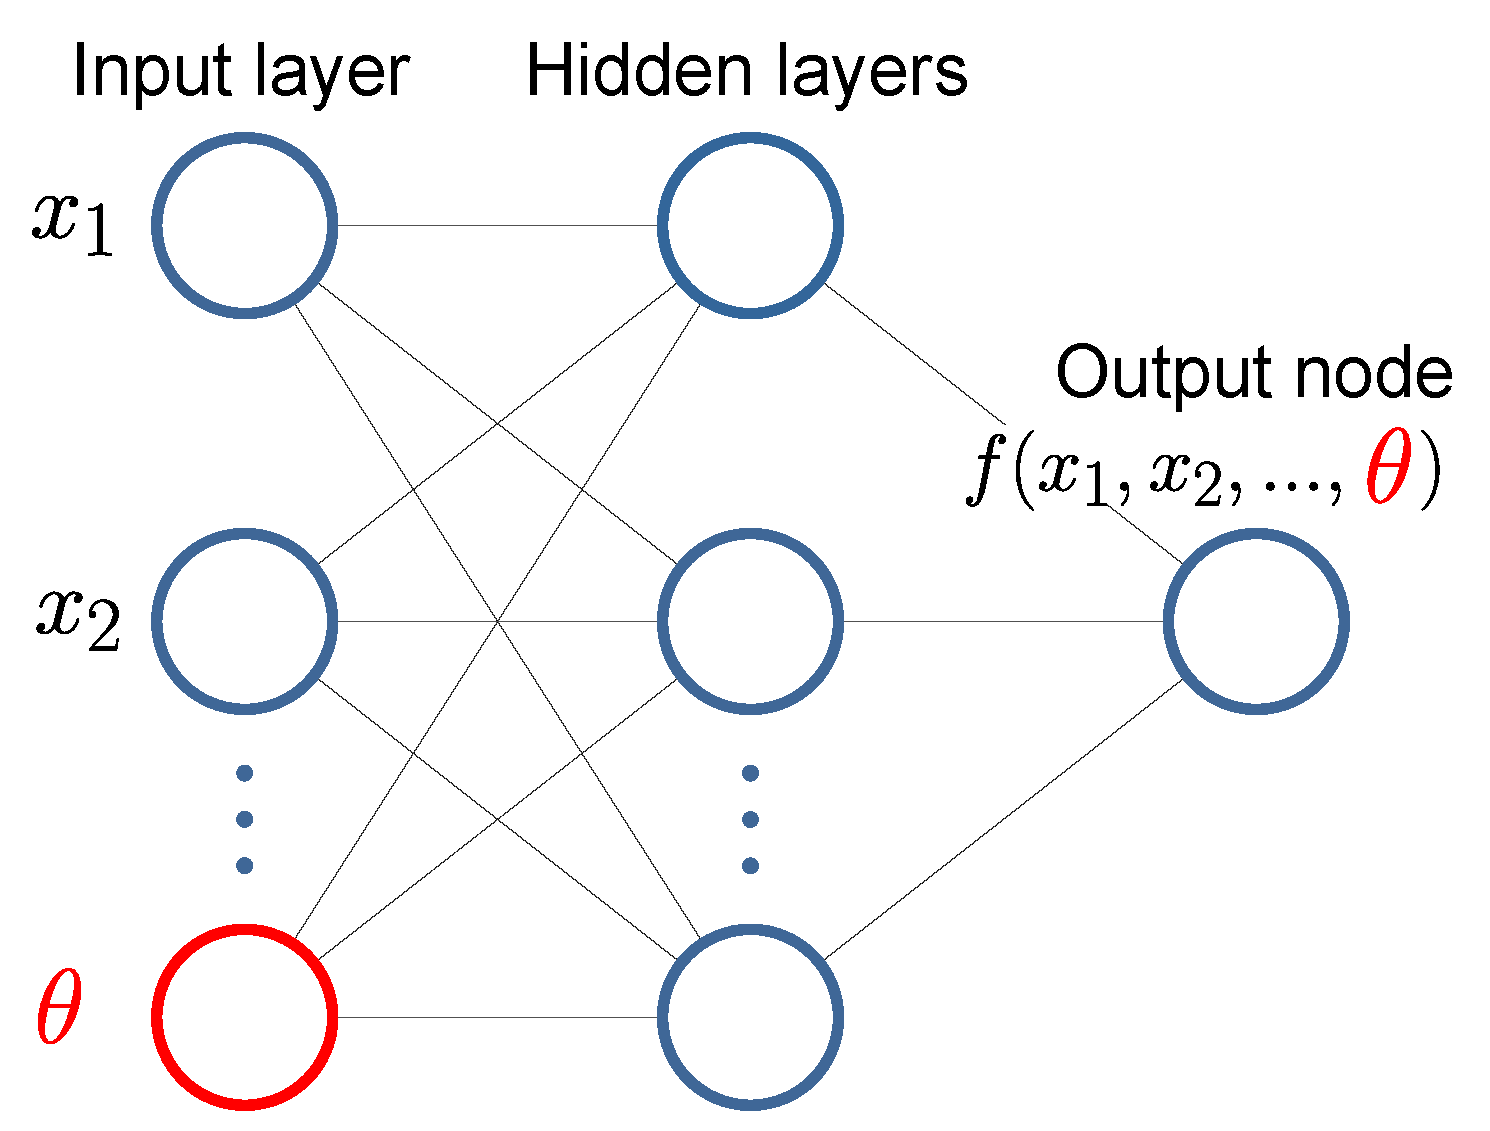
\includegraphics[width=0.75\textwidth]{ML/nntheta.pdf}
    \caption{
        Simple schematic of a fully connected feed-forward Neural network with input features $x_1, x_2,...$ as well as an input parameter $\theta$, such as response $f$ depends on the parameter.
    }
    \label{ML:PNN}
    \end{center}
\end{figure}

\subsection{Boosted decision trees}

Boosted decision trees (BDTs) were one of the most commonly used multivariate technique in the last decade of high energy physics, before NNs became more accessible and popular. \\

BDTs are used for various problem sets like NNs, as object identification or signal/background discrimination. Implementation are in typical \acrshort{ATLASlabel} software, ROOT~\cite{BRUN199781} via the TMVA~\cite{TMVA} package and more widely in python via scikit-learn~\cite{scikit-learn} or xgboost~\cite{Chen_2016}.\\

The unit of a BDT is a decision tree, depicted in Figure~\ref{ML:BDT}. The structure is like a tree, as the name suggests, with branches connected via nodes. A cut on a specific input is made at each node, repeated until a stop criterion is met. The most usual criteria are that the minimum events in a leaf is reached or that the maximum amount of cuts is reaches (maximal tree depth). The decision tree alone is a weak learner and very sensitive to small changes in the training data, while an ensemble of weak learning leads to a powerful and robust model.
 
\begin{figure}[htbp]
    \RawFloats
    \begin{center}
    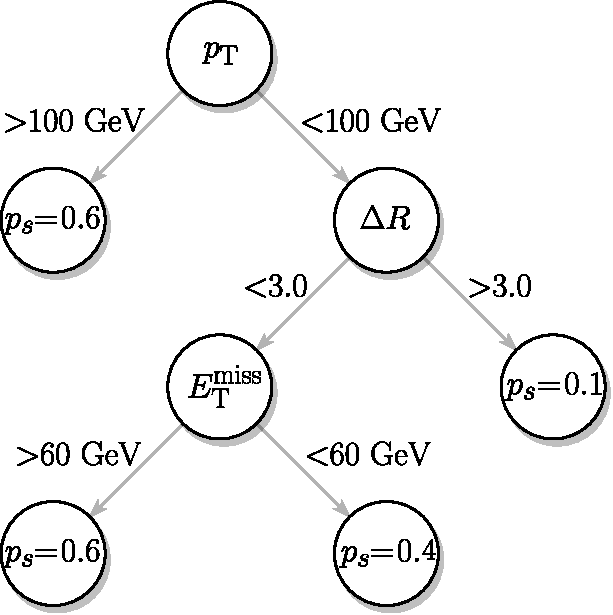
\includegraphics[width=0.75\textwidth]{ML/BDTtree.pdf}
    \caption{
        Schematic representation of a decision tree trained on a dataset composed of signal and background events with example training variables and cuts. The output of the tree is the probability that each event has of being generated by signal, values above (below) 0.5 correspond to signal-like (background-like) events.
    }
    \label{ML:BDT}
    \end{center}
\end{figure}

Boosting is one technique to ensemble trees, which combines the response of the single decision trees into a single discriminant,

\begin{equation}
    \text{P}_{\text{model}} = \sum_{n=1}^N \alpha_n \text{P}_{\text{tree}}^{(n)}(\mathbf{x_i})
\end{equation}

Different boosting methods are widely available and the most popular for classification are Gradient Boosting (GradBoost) and Adaptive Boosting (AdaBoost)~\cite{FREUND1997119}. A GradBoost BDT~\cite{Chen_2016} consists on training individual trees sequentially computing the loss function, typically $E_{MSE}$, and the contribution of the next tree is added to the ensemble weighted such as the loss function is minimised,

\begin{equation}
    E_n = E\left(\text{P}_{\text{model}}^(n-1)(\mathbf{x_i})+\gamma_n \text{P}_{\text{tree}}^{(n)}(\mathbf{x_i})\right)
\end{equation}

AdaBoost is a specific case in which the weight of the events wrongly classified for a given tree is increased to have an impact in the loss function minimisation, hence increasing the learning in challenging phase-spaces. Nevertheless, this can yield to a model sensitive to statistical deviations of the dataset or outlier events.


\section{Profile likelihood fit}
\label{sec:profilelikelihoodfit}

In order to test the compatibility between data and the \acrshort{MClabel} simulations, statistical methods in the context of hypothesis testing need to be introduced. The profile likelihood fit is a statistical tool used in this thesis to extract a measurement for the amount of the signal targeted in the analysis. When the presence of signal is not significant, upper limits are extracted based on the asymptotic formulation~\cite{Cowan_2011}. In this section, the profile likelihood fit method is presented with the necessary concepts in the context of a \acrshort{BSMlabel} search.
The technical implementation is provided by the RooStat framework~\cite{10.48550/arxiv.1009.1003}.\\

The fundamental idea behind hypothesis testing is to compare the agreement of the experimental data between two hypotheses and quantify which hypothesis can be discarded with a certain level of confidence. The two hypotheses to be compared are: the null-hypothesis $H_0$, the~\acrshort{SMlabel} without new physics; and the alternative hypothesis $H_\mu$, which accounts for \acrshort{BSMlabel} interactions. The $\mu$ refers to the signal strength, commonly referred as parameter of interest (POI), which is a normalisation factor for the targeted signal that can be expressed as,

\begin{equation}
    \mu = \frac{\sigma}{\sigma_{ref}}
\end{equation}

where $\sigma$ is arbitrary and $\sigma_{ref}$ a reference value, typically a benchmark value from a theory or an expected sensitivity, like 1~pb. Hence, $H_\mu$ can be evaluated with a continuos spectrum of signal strengths, and will approach the \acrshort{SMlabel} hypothesis ($H_0$) for $\mu\to0$, the agreement is checked for $H_\mu$ with a continuous spectrum of signal strengths, which will approach the \acrshort{SMlabel}, $H_0$, for $\mu=0$.\\

Given a binned data distribution with $n_i$ events for a bin $i$, the expected value of $n_i$ can be expressed as,

\begin{equation}
    E[n_i(\mu,\mathbf{b},\boldsymbol{\theta})] = \mu\cdot s_i(\boldsymbol{\theta}) + \sum_{k_{\alpha}\in\mathbf{k}}k_\alpha\cdot b_{\alpha,i}(\boldsymbol{\theta})
\end{equation}

with $s_i$ the predicted signal events, $b_{\alpha,i}$ the predicted background events of the process $\alpha$. The normalisation factor $k_\alpha$ affects the background process $\alpha$, analogous to $\mu$. Typically, $k_\alpha$ is introduced only for the most relevant backgrounds. The rest of the processes are normalised to their predicted cross-sections and the corresponding $k_\alpha$ is fixed to one. The nuisance parameters $\boldsymbol{\theta}$ are additional degrees of freedom which correspond to the systematic uncertainties acting both on the shape and normalisation of all processes. Their central value is defined to be zero and the deviation with respect to the original value is referred to as pull, where a deviation of $\pm$1 corresponds to a variation of one standard deviation.\\

The fit procedure allows the reduction of the impact of systematic uncertainties, especially by taking advantage of the highly populated background-dominated bins included in the fit. This requires a good understanding of the background and the systematic effects. To verify the improved background prediction, fits under the background-only hypothesis are typically performed, and differences between the data and the post-fit background prediction are checked using selections and physical variables other than the ones used in the fit.\\

The binned likelihood function is given as
\begin{equation}
    \mathscr{L}(\mu,\mathbf{k},\boldsymbol{\theta}) = \prod_i^N \frac{ (E[n_i(\mu,\mathbf{b},\boldsymbol{\theta})])^{n_i}}{n_i!}e^{E[n_i(\mu,\mathbf{b},\boldsymbol{\theta})]}\prod_{\theta_j\in\boldsymbol{\theta}}P(\theta_j)
\end{equation}

which corresponds to a product of Poisson probabilities for all $N$ bins and the penalty terms of all nuisance parameters. The form $P(\theta_j)$ are generally Gaussian distributions for each systematic uncertainties and Poisson distributions for the statistical uncertanty of each bin, that are introduced in the likelihood to penalise large deviations.\\


The optimal $\mu$, $\mathbf{k}$ and $\boldsymbol{\theta}$ are obtained from the fit to data that maximises the agreement between data and the prediction.

The optimal test statistic to perform the fit is the likelihood ratio, %https://link.springer.com/chapter/10.1007/978-1-4612-0919-5_5

\begin{equation}
    \lambda_\mu = \frac{\mathscr{L}(\mu, \hat{\hat{\mathbf{k}}},\hat{\hat{\boldsymbol{\theta}}})}{\mathscr{L}(\hat{\mu}, \hat{\mathbf{k}},\hat{\boldsymbol{\theta}})}
\end{equation}

with the single-hat parameters that maximise likelihood while $\hat{\hat{\mathbf{k}}},\hat{hat{\boldsymbol{\theta}}}$ those that maximise the likelihood for a given $\mu$. As the likelihoods are products of several terms smaller than one, a more stable test statistic is the negative log-likelihood,

\begin{equation}
    q_\mu = -2\ln\lambda_\mu
\end{equation}

For the purpose of setting upper limits on the signal production, some special cases are defined depending on $\mu$ and $\hat{\mu}$. If $\hat{\mu}$ is negative, i.e. the fitted signal has a negative normalisation, the modified test statistic assumes signal to be only positive: $\tilde{q}(\mu)=-2\ln\frac{\mathscr{L}(\mu, \hat{\hat{\mathbf{k}}},\hat{\hat{\boldsymbol{\theta}}})}{\mathscr{L}(0, \hat{\hat{\mathbf{k}}},\hat{\hat{\boldsymbol{\theta}}})}$, where the parameters in the denominator optimise the likelihood for $\mu=0$. Another exception is to set the modified test statistic to 0 for $\hat{\mu}>\mu$, as signal below the observed measurement is in complete agreement with the hypothesis.\\

The level of agreement between data and predictions for a given signal strength is quantified by computing the p-value $p_\mu$, which is the probability of the measured data being a deviation from the assumed $H_\mu$,

\begin{equation}
    p_\mu = \int_{q_{\mu,obs}}^\infty f(q_\mu|H_\mu)dq_\mu
\end{equation}

where $f(q_\mu|H_\mu)$ is the probability density function of $q_\mu$ under the assumption of $H_\mu$. The significance $Z=\Phi^{-1}(1-p_\mu)$ (being $\Phi$ the cumulative Gaussian distribution) is often preferred to quantify the level of disagreement in terms of sigma deviations. Typically, an alternative hypothesis is rejected at 1.64$\sigma$ ($p_\mu=0.05$) and the background-only at 5$\sigma$ ($p_0=2.87\cdot10^{-7}$).\\

Normally, searches are dedicated to very small signals and poorly separated from the background. Rejecting the null hypothesis at a fixed probability as mentioned, leads to exclude signals with very low statistics not really targeted by the analysis~\cite{JUNK1999435}. The CL$_{s}$ method solves this issue, which defines,

\begin{equation}
    \text{CL}_{s}=\frac{p_\mu}{1-p_0}
\end{equation}

which is the previous p-value, which any bad compatibility benefits the background-only hypothesis; normalised to the confidence level of the background-only hypothesis, which is closer to 1 when the measurement is not compatible with the background. In general, the exclusion limits obtained with this method are conservative.

